\chapter{Software Testing}\label{ch:testing}
\section{Objectives, Scope and Integrity}
Testing targets validation, policy, widgets, workflow transitions, authorization, concurrency and graceful failure across all seven modules. Evidence was inspected in \texttt{test/account\_policy\_test.dart}, \texttt{test/widget\_test.dart}, other Flutter tests, and \texttt{functions/test}. The repository records earlier successful runs in \texttt{docs/verification.md}; however, a fresh \texttt{flutter test --no-pub} attempt during this update did not complete and was interrupted. A fresh \texttt{npm test} in \texttt{functions} stopped before test execution because the local installation could not resolve \texttt{firebase-admin/app}. Historical evidence is labelled, and unexecuted scenarios are not promoted to Pass. The account-policy test still expects \texttt{pending} to be denied while current policy denies only suspended/rejected; it requires correction and rerun.
\section{Approach and Environment}
Unit/widget tests cover validators, eligibility, policy and responsive forms. Firebase Emulator Suite tests cover rules and callable workflows without production data. Physical devices are required for OTP, GPS, push delivery, background handling and complete multi-user evidence.
\begin{landscape}\scriptsize
\begin{longtable}{p{1.2cm}p{2.2cm}p{3cm}p{2.5cm}p{3.3cm}p{3.2cm}p{1.6cm}p{3cm}}
\caption{Module test cases and evidence}\label{tab:testcases}\\
\toprule Test Case ID&Module&Test Scenario&Input&Expected Result&Actual Result&Status&Evidence/Screenshot Reference\\\midrule\endfirsthead
\toprule Test Case ID&Module&Test Scenario&Input&Expected Result&Actual Result&Status&Evidence/Screenshot Reference\\\midrule\endhead
AUTH-01&Authentication Module&Valid signup&Unique valid form&Auth user and approved profile&Needs configured backend/device&Not Executed&[SCREENSHOT PLACEHOLDER: Signup]\\
AUTH-02&Authentication Module&Approval-free login&Valid non-blocked account&Role screen opens&Source allows all except rejected/suspended; fresh suite incomplete&Not Executed&\texttt{account\_policy.dart}\\
AUTH-03&Authentication Module&Blocked account&Suspended/rejected status&Access denied&Fresh run incomplete&Not Executed&\texttt{account\_policy\_test.dart}\\
AUTH-04&Authentication Module&Malformed form&Bad email/weak password&Inline validation&Recorded in prior Flutter run&Pass&\texttt{docs/verification.md}\\
AUTH-05&Authentication Module&Phone OTP&Valid/invalid OTP&Link or explicit error&Needs device/Firebase Phone Auth&Not Executed&[SCREENSHOT PLACEHOLDER: OTP]\\
DON-01&Donor Module&Eligibility interval&Recent/old dates&Correct eligibility&Recorded prior unit tests&Pass&\texttt{widget\_test.dart}\\
DON-02&Donor Module&Accept request&Eligible compatible donor&Atomic assignment&Historical emulator pass&Pass&\texttt{functions/test/emulator.test.js}\\
DON-03&Donor Module&Reject invalid donor&Wrong group/busy donor&No mutation&Historical backend pass&Pass&Backend tests/verification record\\
DON-04&Donor Module&Responsive UI&Three viewport sizes&No overflow&Visual evidence outstanding&Not Executed&[SCREENSHOT PLACEHOLDER: Donor UI]\\
REC-01&Receiver Module&Create request&Valid two-unit form&Open request/event&Historical emulator pass&Pass&\texttt{emulator.test.js}\\
REC-02&Receiver Module&Invalid request&Bad units/deadline/location&Reject without write&Fresh execution unavailable&Not Executed&[SCREENSHOT PLACEHOLDER: Validation]\\
REC-03&Receiver Module&Cancel request&Assigned open request&Cancel and release donors&Historical emulator pass&Pass&\texttt{docs/verification.md}\\
REC-04&Receiver Module&Create SOS&Valid emergency form&Linked SOS/request&Needs deployed callable&Not Executed&[SCREENSHOT PLACEHOLDER: SOS]\\
NOT-01&Notification Module&Read/empty state&Notification/no data&Correct state/update&Needs app/backend&Not Executed&[SCREENSHOT PLACEHOLDER: Notifications]\\
NOT-02&Notification Module&Urgent push&Valid token/request&Device receives FCM&Needs deployed FCM/device&Not Executed&[SCREENSHOT PLACEHOLDER: Push]\\
NOT-03&Notification Module&Denied/stale token&No permission/invalid token&Core workflow survives&Not device-tested&Not Executed&Device log pending\\
RWD-01&Reward and Certificate Module&Confirm twice&Same request/donor&One donation/award&Historical idempotency pass&Pass&\texttt{emulator.test.js}\\
RWD-02&Reward and Certificate Module&Certificate&Confirmed donation&PDF/upload or clear error&Needs Storage/device&Not Executed&[SCREENSHOT PLACEHOLDER: PDF]\\
RWD-03&Reward and Certificate Module&Forged reward&Client write&Rules deny&Historical rules pass&Pass&\texttt{policy.test.js}\\
ADM-01&Admin Module&Admin login&Auth user with admin role&Dashboard opens&Needs configured admin&Not Executed&[SCREENSHOT PLACEHOLDER: Admin]\\
ADM-02&Admin Module&Non-admin action&Donor calls admin function&Deny&Historical authorization pass&Pass&Backend tests\\
ADM-03&Admin Module&Search/filter&Query/status/role&Correct list/states&Manual evidence outstanding&Not Executed&[SCREENSHOT PLACEHOLDER: Filters]\\
ADM-04&Admin Module&Status action&Target/reason&Update and audit&Manual backend evidence outstanding&Not Executed&[SCREENSHOT PLACEHOLDER: Action]\\
MAP-01&Mapping and Distance Module&Radius search&Known coordinates&Ordered in-radius donors&Fresh run incomplete&Not Executed&\texttt{nearbyDonors.js}\\
MAP-02&Mapping and Distance Module&Consent/eligibility&Disabled/ineligible donor&Exclude donor&Historical backend pass&Pass&Backend tests\\
MAP-03&Mapping and Distance Module&Permission denied&Location denied&Fallback/error shown&Needs device&Not Executed&[SCREENSHOT PLACEHOLDER: Permission]\\
MAP-04&Mapping and Distance Module&Routing outage&OSRM timeout&Distance remains; ETA omitted&Not network-tested&Not Executed&Device log pending\\
\bottomrule\end{longtable}\end{landscape}
\section{Module Assessments}
\subsection{Authentication Module} Positive and negative cases must cover credentials, blocked states and non-admin access. The stale pending-status assertion is a known maintenance issue.
\subsection{Donor Module} Historical policy/emulator evidence covers compatibility, eligibility, assignment and forgery resistance; visual evidence remains.
\subsection{Receiver Module} Creation, cancellation and concurrency have historical emulator evidence; SOS propagation needs deployment testing.
\subsection{Notification Module} Token/UI logic exists, but foreground/background receipt and permissions require devices.
\subsection{Reward and Certificate Module} Idempotency has historical backend evidence; PDF upload/share and QR content require manual evidence.
\subsection{Admin Module} Rules/functions enforce roles; responsive UI, filters, dialogs, exports and audit visibility need configured-admin testing.
\subsection{Mapping and Distance Module} Haversine policy exists; GPS accuracy, permission handling and OSRM ETA require field testing.
\section{Visual Test Evidence}
The following figures document the supplied application states used for visual inspection. They are evidence of the rendered screens and workflow checkpoints, not a substitute for automated execution or device-level testing. The observed values are reproduced exactly as shown in the screenshots.

\begin{figure}[H]\centering
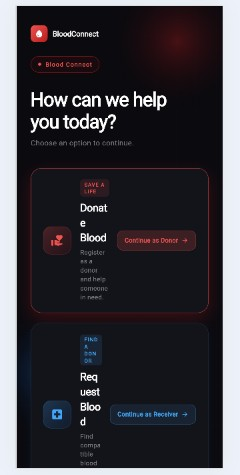
\includegraphics[width=0.42\textwidth,height=0.55\textheight,keepaspectratio]{Figures/screenshots/role_selection.jpeg}
\caption{Role-selection screen used to inspect donor and receiver navigation entry points.}\label{fig:test-role-selection}
\end{figure}

\begin{figure}[H]\centering
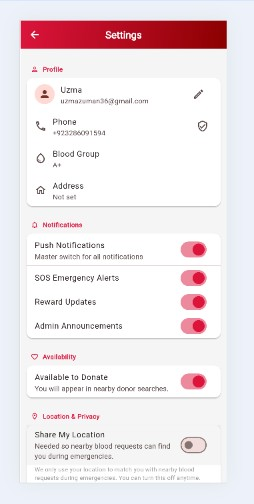
\includegraphics[width=0.42\textwidth,height=0.55\textheight,keepaspectratio]{Figures/screenshots/settings.jpeg}
\caption{Settings screen used to inspect profile data, notification controls and donation availability.}\label{fig:test-settings}
\end{figure}

\begin{figure}[H]\centering
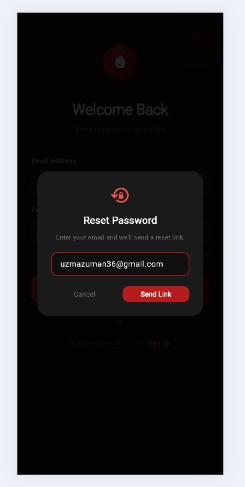
\includegraphics[width=0.42\textwidth,height=0.55\textheight,keepaspectratio]{Figures/screenshots/reset_password.jpeg}
\caption{Reset-password dialog used to inspect input presentation and the reset-link action.}\label{fig:test-reset-password}
\end{figure}

\begin{figure}[H]\centering
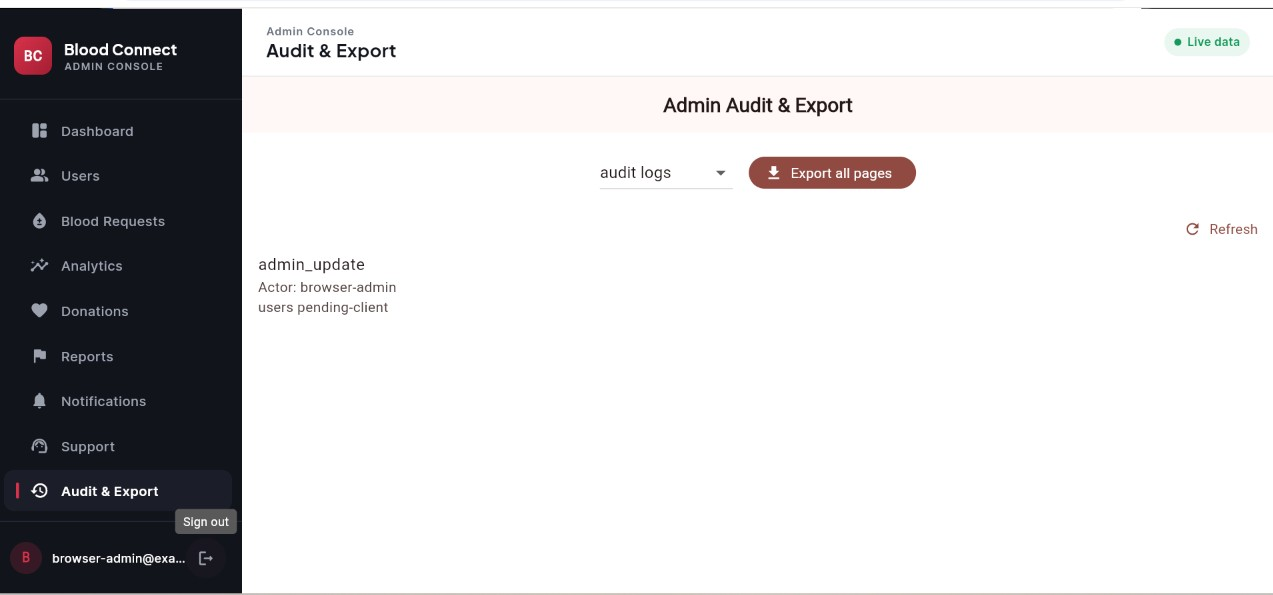
\includegraphics[width=0.95\textwidth,height=0.55\textheight,keepaspectratio]{Figures/screenshots/admin_audit.jpeg}
\caption{Admin audit view used to inspect audit-log visibility and export controls.}\label{fig:test-admin-audit}
\end{figure}

The supplied email-link and email-verified images provide evidence of the external Firebase email-verification step. They do not prove delivery reliability for all accounts; that remains a device and backend test requirement. Similarly, the donor dashboard and administrator screenshots support responsive visual review, while the test matrix correctly leaves automated and production-dependent cases as 
\textit{Not Executed} where no execution record was supplied.
\section{Security, Limitations and Summary}
Emulator tests target owner/participant/admin boundaries, forged writes, transitions, cancellation and concurrent confirmation. Production rules, indexes, App Check and deployed functions still require comparison before release. No fresh full Flutter, backend, or physical-device test run completed during this edit: the Flutter process stalled and the Node test process lacked its installed Firebase Admin dependency. Remaining evidence includes dependency restoration, current suite reruns, two-device flows, OTP, FCM, GPS, certificates, admin actions and responsive screenshots; Table~\ref{tab:testcases} uses \textit{Not Executed} where current evidence is absent.
